\documentclass[11pt]{article}
\usepackage[toc,page]{appendix}
\usepackage{amsmath, amssymb}
\usepackage[utf8]{inputenc}
\usepackage[T1]{fontenc}
\usepackage[style=apa,backend=biber]{biblatex}
%\usepackage{biblatex}
\addbibresource{references.bib}
\usepackage{graphicx}
\usepackage{tikz}
\usetikzlibrary{automata,positioning,shapes.geometric, arrows.meta, fit, backgrounds, calc, chains}
\graphicspath{./images/Easy_Pictures/SAR_ADD_Rounding}%\usepackage{kpfonts}
\usepackage{float}
\usepackage[margin=1in]{geometry}
\usepackage{cancel}
\usepackage{epsfig}
\usepackage{tikz-3dplot}
\usepackage{darkmode}
\usepackage{dirtytalk}
\usepackage{longtable,booktabs,array}
\usepackage{calc} % for calculating minipage widths
\usepackage[utf8]{inputenc}
\usepackage[T1]{fontenc}
\usepackage{xcolor}
\usepackage{listings}


\usepackage{etoolbox}
\usepackage{hyperref}
\hypersetup{
    colorlinks=true,
    linkcolor=blue,
    filecolor=magenta,      
    urlcolor=cyan,
    pdftitle={Hermeneutic Calculator},
    citecolor=blue,
    }


\urlstyle{same}

\lstdefinestyle{htmlStyle}{
    language=HTML,
    basicstyle=\ttfamily\small,
    keywordstyle=\color{blue}\bfseries,
    commentstyle=\color{gray}\itshape,
    stringstyle=\color{red},
    breaklines=true,
    frame=single,
    numbers=left,
    numberstyle=\tiny\color{gray},
    columns=fullflexible,
}
\lstdefinelanguage{HTML}{
  keywords={<!DOCTYPE, html, head, title, body, h1, h2, h3, p, div, span, a, img, ul, li, table, tr, td, th, style, link, script},
  sensitive=true,
  comment=[l]{//},
  morecomment=[s]{/*}{*/},
  morestring=[b]',
  morestring=[b]"
}
\lstset{style=htmlstyle, language=html}
% Updated to explicitly pass the language option
%\lstinputlisting[style=htmlstyle, language=html]{./html/example.html}
%\usepackage{tocloft}

% Optional: define some custom colors
\definecolor{sliceRed}{RGB}{225,224,91} % matching "varyellow" from your code
\definecolor{linkYellow}{RGB}{255,215,0}  % a golden yellow
\tdplotsetmaincoords{70}{110}

\title{Addition Strategies: Rounding and Adjusting}
\author{Compiled by: Theodore M. Savich}



\begin{document}
\maketitle

\subsection*{Transcript}
Video from \textcite{Carpenter1999}. Strategy descriptions and examples adapted from \textcite{HackenbergCourseNotes}. 
\begin{itemize}
\item \textbf{Teacher:} Lucy has eight fish. She wants to buy five more fish. How many fish will Lucy have then?
 

\item \textbf{Robert:} 13 

\item \textbf{Teacher:} How'd you get the 13?

\item \textbf{Robert:} I just took the eight out. And then I, if she had ten fish, it would have been 15. If she had nine fish, it would have been 14. And if it would have been eight fish, which it was, it would have been 13. So, I just got 13. 

\item \textbf{Teacher:} Did you use those blocks to solve this problem?

\item \textbf{Robert:} Well, I only used eight. I didn't use the other five, though. I used part of it in here (gestures to the mat with the blocks) and part of it in my head. you get 13.
\end{itemize}

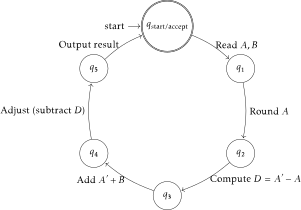
\includegraphics[width=.25\textwidth]{images/Easy_Pictures/SAR_ADD_Rounding/PDF/SAR_ADD_Rounding.pdf}

\noindent \textbf{Notation Representing Robert's Solution:}

\begin{align*}
8 + 5 &= \Box \\
8+2 &= 10\\
10+5 &= 15\\
8+5 &= 15-2\\
8+5 &= 13\\
\end{align*}

\subsubsection*{Description of Strategy:}

 \textbf{Objective:} Rounding for Simplicity:
 We start by changing at least one number to a ``friendlier'' value --- usually rounding it to the closest whole number of bases. For instance, if a number is just a few ones short of a multiple of 10, we can round it up so that it becomes exactly that multiple. This makes the arithmetic easier because we have well-known patterns (adding a full group of 10, for example) where the ones digit remains unchanged and only the tens (or ``base'') digit increases.
 
 \begin{enumerate}
 \item \textbf{The Need to Adjust:} When you round up a number, you are effectively adding a little extra to it. As a result, when you solve the simplified problem, your computed sum is slightly too high compared to the original one. To correct for this, you must subtract the extra amount that you added. Conversely, if you had rounded down (i.e., subtracted some value to simplify the number), then your computed sum would be too low, and you would need to add that amount back in.
 \item \textbf{Why the Inverse Operation?} The principle is simple: whatever operation you use to alter the number for ease of calculation must be undone by the inverse operation to return to the original value.
 \begin{itemize}\item If you \textbf{add} to round a number up, you must \textbf{subtract} later to adjust.
 \item If you \textbf{subtract} to round a number down, you must \textbf{add} back the same amount after solving.
 \end{itemize}
 This two-step process—first simplifying via rounding and then adjusting—helps you manage complex addition while keeping the final answer accurate to the original numbers.
\end{enumerate}
 
 
 
 
 
 

\subsection*{Rounding and Adjusting}

\subsubsection*{Description of Strategy}

\begin{itemize}
    \item \textbf{Objective:} Round one addend to a convenient number (usually a base multiple), perform the addition, then adjust the result.
    \item \textbf{Example:} $46 + 37$
    \begin{itemize}
        \item Round $46$ up to $50$ (adding $4$).
        \item Add: $50 + 37 = 87$.
        \item Adjust: Subtract the $4$ added earlier: $87 - 4 = 83$.
    \end{itemize}
\end{itemize}

\subsubsection*{Automaton Type}
\textbf{Pushdown Automaton (PDA)}: Needed to remember the adjustment amount.

\subsubsection*{Automaton Description}

\begin{itemize}
    \item \textbf{States:}
    \begin{enumerate}
        \item $q_0$: Start state.
        \item $q_1$: Read inputs and decide which number to round.
        \item $q_2$: Round the chosen number.
        \item $q_3$: Compute the adjustment.
        \item $q_4$: Perform the addition with the rounded number.
        \item $q_5$: Adjust the sum.
        \item $q_{accept}$: Accept state; output the final result.
    \end{enumerate}
    \item \textbf{Transitions:}
    \begin{itemize}
        \item $q_0 \rightarrow q_1$: Read $A$ and $B$; decide to round $A$.
        \item $q_1 \rightarrow q_2$: Round $A$ to $A'$.
        \item $q_2 \rightarrow q_3$: Calculate adjustment $D = A' - A$.
        \item $q_3 \rightarrow q_4$: Add $A'$ and $B$.
        \item $q_4 \rightarrow q_5$: Adjust the sum by subtracting $D$.
        \item $q_5 \rightarrow q_{accept}$: Output the adjusted sum.
    \end{itemize}
\end{itemize}


We define the PDA 
\[
M = (Q,\Sigma,\Gamma,\delta,q_0,Z_0,F)
\]
where:
\begin{itemize}
    \item \(Q = \{q_0,\, q_1,\, q_2,\, q_3,\, q_4,\, q_5,\, q_{\text{accept}}\}\) is the set of states.
    \item \(\Sigma = \{0,1,2,3,4,5,6,7,8,9,+\}\) is the input alphabet (for example, representing inputs like ``46+37'').
    \item \(\Gamma = \{Z_0\} \cup \{x \mid x \in \mathbb{Z}\}\) is the stack alphabet, where \(Z_0\) is the initial stack symbol and an integer \(x\) represents the adjustment amount.
    \item \(q_0\) is the start state.
    \item \(Z_0\) is the initial stack symbol.
    \item \(F = \{q_{\text{accept}}\}\) is the set of accepting states.
\end{itemize}

The transition function 
\[
\delta: Q \times (\Sigma \cup \{\varepsilon\}) \times \Gamma \to \mathcal{P}(Q \times \Gamma^*)
\]
is defined by the following transitions:
\begin{enumerate}
    \item \(\delta\Bigl(q_0,\, \text{``}A,B\text{''},\, Z_0\Bigr) = \{(q_1,\, Z_0)\}\). 
    \item \(\delta(q_1,\, \varepsilon,\, Z_0) = \{(q_2,\, Z_0)\}\) \quad (Round \(A\) to \(A'\)).
    \item \(\delta(q_2,\, \varepsilon,\, Z_0) = \{(q_3,\, D\,Z_0)\}\) \quad (Compute \(D = A' - A\) and push \(D\) onto the stack).
    \item \(\delta(q_3,\, \varepsilon,\, D) = \{(q_4,\, D)\}\) \quad (Perform the addition \(A' + B\)).
    \item \(\delta(q_4,\, \varepsilon,\, D) = \{(q_5,\, \varepsilon)\}\) \quad (Adjust the sum by subtracting \(D\); pop \(D\) from the stack).
    \item \(\delta(q_5,\, \varepsilon,\, Z_0) = \{(q_{\text{accept}},\, Z_0)\}\) \quad (Output the final result).
\end{enumerate}

\subsection*{Automaton Diagram for Rounding and Adjusting}

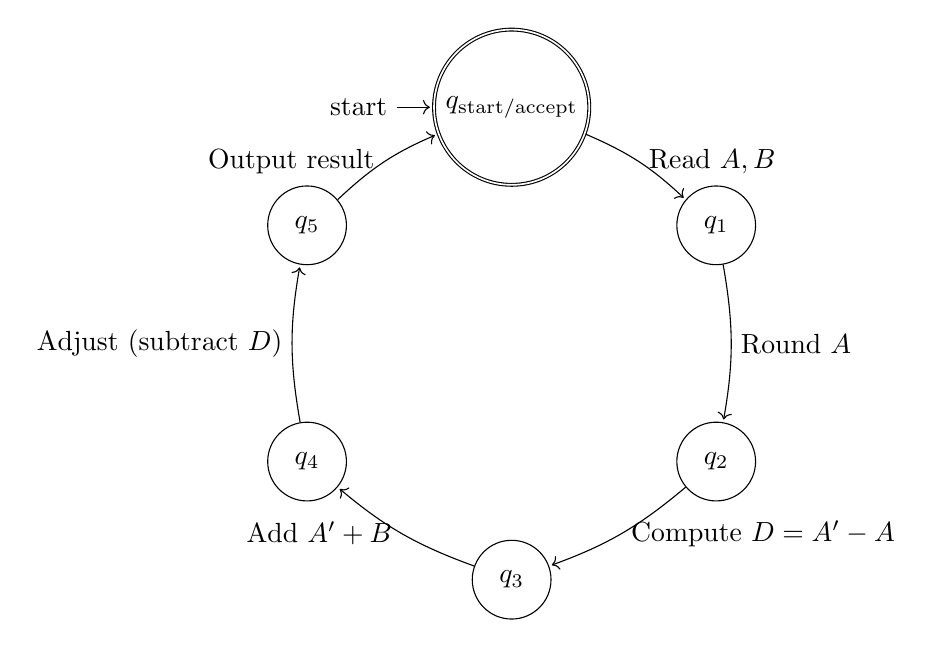
\begin{tikzpicture}[
    shorten >=1pt,
    node distance=2.5cm,
    on grid,
    auto,
    every state/.style={minimum size=1cm}
]
    % Calculate positions for hexagon vertices
    \def\radius{3cm}
    \def\startangle{90}
    
    % States positioned in a hexagon
    \node[state, initial, accepting] (q0) at (\startangle:\radius) {$q_{\text{start/accept}}$};
    \node[state] (q1) at (\startangle-60:\radius) {$q_1$};
    \node[state] (q2) at (\startangle-120:\radius) {$q_2$};
    \node[state] (q3) at (\startangle-180:\radius) {$q_3$};
    \node[state] (q4) at (\startangle-240:\radius) {$q_4$};
    \node[state] (q5) at (\startangle-300:\radius) {$q_5$};
    
    % Transitions
    \begin{scope}[on background layer]
        \path[->]
            (q0) edge[bend left=10] node[right] {Read \(A, B\)} (q1)
            (q1) edge[bend left=10] node[right] {Round \(A\)} (q2)
            (q2) edge[bend left=10] node[right] {Compute \(D = A' - A\)} (q3)
            (q3) edge[bend left=10] node[left] {Add \(A' + B\)} (q4)
            (q4) edge[bend left=10] node[left] {Adjust (subtract \(D\))} (q5)
            (q5) edge[bend left=10] node[left] {Output result} (q0);
    \end{scope}
\end{tikzpicture}


\subsubsection*{HTML Implementation}
\lstinputlisting[style=htmlStyle, language=html]{./new_html/SAR_ADD_Rounding.html}

\printbibliography
\end{document}